\chapter{Contexte théorique}
\label{sec:cntxt-thr}

Ce chapitre présente les éléments théoriques nécessaires à la compréhension de ce travail. Après un rappel du Modèle Standard et des propriétés des hadrons, nous introduisons les particules étudiées ainsi que les enjeux liés à leur détection dans les calorimètres hadroniques.

\section{Le Modèle Standard de la physique des particules}

Le \textit{Modèle Standard} (MS) constitue aujourd'hui le cadre théorique de référence pour décrire les particules élémentaires et trois des quatre interactions fondamentales : l'interaction forte, l'interaction faible et l'interaction électromagnétique. La gravitation n'y est pas incluse \cite{Griffiths2008, HalzenMartin1984}.

Il repose sur la symétrie de jauge :

\[
SU(3)_C \times SU(2)_L \times U(1)_Y,
\]

où :

\begin{itemize}
    \item \(SU(3)_C\) décrit la chromodynamique quantique (QCD), théorie de l'interaction forte ;
    \item \(SU(2)_L \times U(1)_Y\) décrit le secteur électrofaible \cite{PeskinSchroeder1995} ;
    \item après brisure spontanée de symétrie via le mécanisme de Brout--Englert--Higgs, l'électromagnétisme émerge via le groupe \(U(1)_{\mathrm{em}}\), et les particules acquièrent leur masse.
\end{itemize}

Le Modèle Standard a été validé expérimentalement avec une précision remarquable, culminant avec la découverte du boson de Higgs en 2012 au LHC \cite{ATLASHiggs2012, CMSHiggs2012}.

\begin{figure}[!ht]
    \centering
    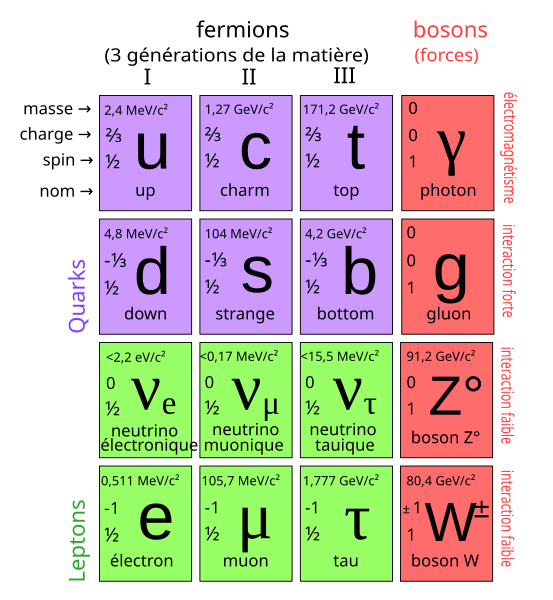
\includegraphics[width=0.5\linewidth]{img/ms.png}
    \caption{Particules élémentaires décrites par le Modèle Standard \cite{pdg2024}.}
    \label{fig:SM}
\end{figure}

\section{Constituants fondamentaux}

Les particules du Modèle Standard se répartissent en deux grandes catégories : les fermions, constituants de la matière, et les bosons, médiateurs des interactions.

\subsection{Fermions}

Les fermions de spin \(1/2\) obéissent à la statistique de Fermi-Dirac. Ils se divisent en :

\begin{itemize}
    \item \textbf{Leptons} : électron \(e\), muon \(\mu\), tau \(\tau\) et leurs neutrinos associés ;
    \item \textbf{Quarks} : \(u,\,d,\,c,\,s,\,t,\,b\), porteurs de charge de couleur et soumis à l'interaction forte.
\end{itemize}

Ils sont organisés en trois générations de masses croissantes. La matière ordinaire est essentiellement constituée des fermions de première génération.

\subsection{Bosons de jauge}

Les interactions fondamentales sont médiées par des bosons de spin 1 :

\begin{itemize}
    \item photon \(\gamma\) : interaction électromagnétique ;
    \item bosons \(W^\pm\) et \(Z^0\) : interaction faible \cite{pdg2024} ;
    \item gluons : interaction forte.
\end{itemize}

\subsection{Boson de Higgs}

Le boson de Higgs est une particule scalaire de spin 0, responsable de la brisure spontanée de la symétrie électrofaible et de la génération des masses des particules.

\section{Hadrons et interaction forte}

Dans le contexte de la calorimétrie hadronique, les particules observées expérimentalement sont principalement des états liés de quarks, appelés hadrons.

La QCD décrit l'interaction forte entre quarks et gluons. Elle est caractérisée par deux propriétés fondamentales \cite{PeskinSchroeder1995} :

\begin{itemize}
    \item \textbf{Confinement de couleur} : les quarks ne sont jamais observés isolément ;
    \item \textbf{Liberté asymptotique} : le couplage fort diminue à haute énergie.
\end{itemize}

On distingue principalement deux familles d'hadrons \cite{pdg2024} :

\begin{itemize}
    \item \textbf{Baryons} (\(qqq\)) : proton, neutron, etc. ;
    \item \textbf{Mésons} (\(q\bar{q}\)) : pions, kaons, etc.
\end{itemize}

Leur interaction avec la matière absorbante repose sur des processus nucléaires inélastiques complexes, à l'origine du développement des gerbes hadroniques dans les calorimètres.

\section{Particules d'intérêt de cette étude}

Dans ce travail, nous nous concentrons sur trois espèces hadroniques représentatives, choisies pour leurs signatures calorimétriques distinctes.

Leurs propriétés fondamentales sont résumées dans le Tableau~\ref{tab:hadrons}.

\begin{table}[!ht]
    \centering
    \caption{Propriétés des hadrons étudiés \cite{pdg2024}.}
    \label{tab:hadrons}
    \begin{tabular}{lccccl}
        \hline
        \textbf{Particule} & \textbf{Symbole} & \textbf{Masse (MeV)} &
        \textbf{Charge} & \textbf{Temps de vie} & \textbf{Contenu en quarks} \\
        \hline
        Pion chargé  & \(\pi^-\)  & 139.57  & \(-1\) & \(26.0\)~ns   & \(\bar{u}d\)                        \\
        Proton       & \(p\)      & 938.27  & \(+1\) & stable        & \(uud\)                             \\
        Kaon neutre long & \(K^0_L\) & 497.61 & \(0\) & \(51.2\)~ns  & \(\frac{1}{\sqrt{2}}(d\bar{s}-s\bar{d})\) \\
        \hline
    \end{tabular}
\end{table}

Ces particules présentent des comportements différents dans un calorimètre :

\begin{itemize}
    \item \textbf{Les pions} produisent des gerbes avec une composante électromagnétique significative via la production de \(\pi^0\) ;
    \item \textbf{Les protons} génèrent des gerbes plus hadroniques et généralement plus profondes ;
    \item \textbf{Les kaons neutres longs} n'ionisent pas avant leur première interaction et présentent des signatures distinctes liées à leur étrangeté.
\end{itemize}

La séparation de ces espèces constitue le problème central d'identification de particules (PID) étudié dans ce mémoire.

\section{Lien avec la calorimétrie hadronique}

Dans les expériences de physique des hautes énergies, une fraction importante de l'énergie finale est transportée par des hadrons organisés en jets. La mesure précise de ces jets repose de manière déterminante sur les calorimètres hadroniques.

Les gerbes hadroniques présentent des fluctuations importantes liées aux processus nucléaires inélastiques, à l'énergie invisible et aux fuites, ce qui dégrade la résolution énergétique. Ces limitations constituent une motivation centrale pour le développement de calorimètres à haute granularité.

Le \emph{Semi-Digital Hadron CALorimeter} (SDHCAL), développé au sein de la collaboration CALICE, s'inscrit dans cette approche. Sa granularité fine et sa lecture multi-seuils permettent d'exploiter la structure des gerbes hadroniques de manière détaillée, ouvrant la voie à des méthodes avancées d'identification des particules et de reconstruction d'énergie.